\documentclass[11pt]{article}

\usepackage{fullpage}
\usepackage{url}
\usepackage{graphicx}


\begin{document}

\title{ARM Checkpoint Report}
\author{Group 39\\ \small \textit{Thomas Wong, Steven Chen, Nixon Enraght-Moony, Rickie Ma}}

\maketitle

\section{Group Organisation}

Our group first joined together to work out the structures and the datatypes that we would use, we also implemented the input logic, which was challenging at first. \\
We then split the four functions up to work independently from each other. It wasn't until later we found out that this approach is a bit flawed.\\
Everyone had a different c file to implement their function, which enables parallel coding and made life much easier when dealing with merge requests.\\
We mainly discuss problems in the labs or through WhatsApp, which is a good mix, as some of us are more comfortable working remotely while some prefer to talk face-to-face. Also, all the merge requests are carefully reviewed and voted to ensure no bad code is merged into master. In later tasks I would hope that we split the work more evenly, i.e. people doing easier functions would collaborate with other people to tackle more difficult tasks.

\section{Implementation Strategies}

\subsection{Disassembler}
Before we even started to implement the emulator, we first coded a disassembler that would translate binary files into arm11 assembly referring to the Capstone tools. We also have a dedicated test suite (in \path{/tests}) written in go for the disassembler.

\subsection{Makefile}
Our makefile \path{/src/Makefile} not only contains all the essential bits that is required to build the emulator and the disassembler, it also contains some sanitizers (\textbf{asan}, \textbf{msan}, \textbf{ubsan}) to check errors at runtime. A CLang formatter can also be found here, as well as a command to run the generator for masks written in python. The main makefile \path{/Makefile} also contains the command to start the ruby server for testing.

\subsection{maskgen}
\path{/src/maskgen.py} contains a simple generator for the masking on the 32-bit instruction, it generates the corresponding file \path{/src/lib/mask.c} and its header file \path{/src/include/mask.h}.

\subsection{Structure}
\begin{center}
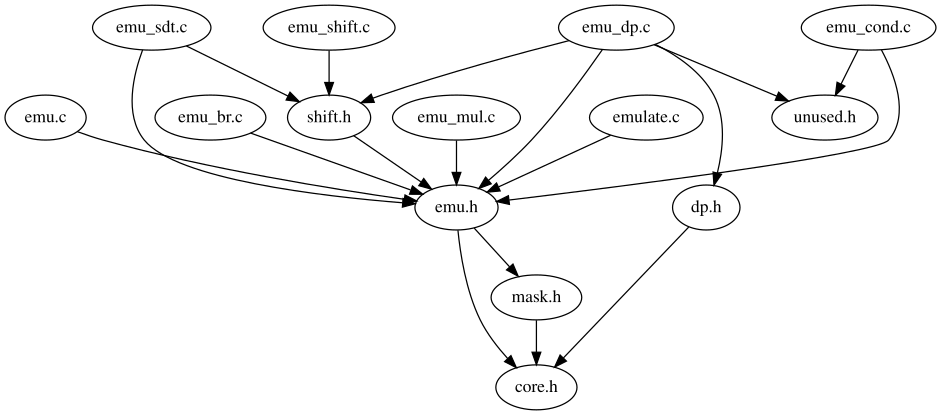
\includegraphics[scale=0.45]{interim/dependency.png}\\
\texttt{Dependency Graph for Emulator}
\end{center}

\begin{itemize}
\item \texttt{emu\_br.c} contains the branch instructions.
\item \texttt{emu\_cond.c} contains the condition codes.
\item \texttt{emu\_dp.c} cotains data processing instructions, implemented by funciton pointers and calls the shifter function in certain cases.
\item \texttt{emu\_mul.c} contains the multiply instructions.
\item \texttt{emu\_sdt.c} contains single data transfer instructions, also supporting GPIO.
\item \texttt{emu\_shift.c} is a helper function for \texttt{emu\_sdt.c} and \texttt{emu\_dp.c}, behaves as a register shifter. This function is also implemented by the use of function pointers.
\item \texttt{emu.c} contains the \texttt{print\_state} function, which outputs the register states and the memory after execution. It also contains the \texttt{emu} function, which parses the instructions into its corresponding function.
\item \texttt{mask.c} contains various diffrenet masks for the 32-bit instructions, which are generated from a python script \texttt{maskgen.py}. The python script along with \texttt{mask.c} and \texttt{mask.h} can be reused in the assembler.
\item The stucture of \textit{CpuState} is defined in \texttt{emu.h}, which consists two arrays of registers and memory.
\end{itemize}
Our team voted and decided not to do the \textit{three stage pipeline approach} based on two reasons, to save memory and to simplify code. 

\section{Further Challenges}
As mentioned before, we had some issues on distributing work, functions such as branch and multiply are largely trivial compare to the others. We would distribute workload more evenly in the assembler part that is yet to come.\\
Also, the extension will challenging, and in order to allocate enough time for the extension, we are planning to start tackling the assembler as soon as possible.

\end{document}

%%% Local Variables:
%%% mode: latex
%%% TeX-master: t
%%% End:
